\subsubsection{Application Programming Interfaces (APIs)}
\label{sec:APIs}

Aufbauend auf dem abgeschlossen Administrationsbereich werden im Folgenden
Application Programming Interfaces, kurz APIs, implementiert. Aufgabe solcher
APIs ist es, Informationen in maschinenleserlicher Form für andere Teilbereiche
des Systems bereitzustellen. Die bereitgestellten Informationen werden von den
aufrufenden Systemen genutzt, um Inhalte dynamisch darzustellen.
In einem Beispiel soll der zuvor vorgestellte Prototyp die Menge der
benachbarten Panoramas über eine solche API beziehen und darauf aufbauend dem
Benutzer die Navigationspfeile entsprechend präsentieren. Die Implementierung
einer API wird nachfolgend an diesem Beispiel erläutert.

Die Realisierung der Schnittstelle vollzieht sich in zwei Schritten.
Zuerst werden die Informationen maschienenleserlich geschrieben und ausgeben. Im
zweiten Schritt werden diese Informationen dann von einem verarbeitenden System
eingelesen und ausgewertet. Das Schreiben von maschinenleserlichen Informationen
hängt stark davon ab, welche Maschine den ausgegeben Text lesen bzw.
interpretieren soll. Im vorliegenden Projekt werden die erstellten APIs
ausschließlich von Javascript-Routinen angefragt, um Inhalte asynchron
nachzuladen. Auf die Bedeutung von asynchronem Nachladen wird später genauer
eingegangen. An dieser Stelle ist lediglich zu beachten, dass die APIs von
Javascript-Routinen angefragt werden. Aus diesem Grund werden die Informationen
der API im JSON-Format dargestellt. JSON steht dabei für "`Javascript Object
Notation"' und ist der de facto Standard für die Kommunikation zwischen
webbasierten Schnittstellen.\footnote{\citet[S.~20]{lubbers2011}} Die
Darstellung im JSON-Format bietet den großen Vorteil, dass innerhalb von
Javascript aus den dargestellten Informationen ein Objekt im Sinne der
objektorientierten Programmierung\footnotemark erstellt werden kann. An dieser
Stelle soll diese Begründung für die Wahl des JSON-Formats ausreichen. Eine
genauere Betrachtung erfolgt im zweiten Schritt der Implementierung der API.
Neben der Klassifikation der API muss noch der darzustellende Inhalt definiert
werden. Für den oben beschriebenen Anwendungsfall müssen hierbei alle Nachbarn
eines gegebenen Panoramas dargestellt werden. Für die Ausrichtung der
Navigationspfeile wird zusätzlich die Himmelsrichtung in Grad jedes Nachbarn
relativ zum Standpunkt des gegeben Panoramas benötigt. Dieser letzte Wert wird
als "`Heading"' bezeichnet und wird bereits bei der Positionierung des
360-Grad-Fotos in der Datenbank gespeichert. Er muss also nur aus der Datenbank
abgefragt werden.

\footnotetext{Die Objektorientierte Programmmierung (OOP) ist
das führende Programmierparadigma für Webanwendungen. Dieses Paradigma
beschreibt eine bestimmte Denkweise für Problemstellungen der Informatik. Für
weitere Einblicke siehe \citet{poetzsch2000}}

Aufbauend auf der vorausgegangenen Beschreibung der API kann diese in PHP
implementiert werden. Dazu wird zunächst das in \verweis{Datenbankentwurf}
beschriebene Tabellenmodell in Bezug auf die darzustellenden Informationen
untersucht. In der \abbildung{Tabellenmodell} ist zu sehen, dass
\textit{heading} ein Attribut der Tabelle \textit{neighbour} ist. Über diese
Tabelle können zu einem gegeben Panorama alle Nachbarn mit entsprechendem
\textit{heading} gefunden werden.
Im Zuge der Implementierung sollen im Folgenden mit Hilfe von PHP über SQL alle
Nachbarn eines gegebenen Panoramas abgefragt werden. Das Ergebnis dieser
Abfrage soll im JSON-Format dargestellt werden. Im \listing{PHP_Nachbar_API}
ist diese Funktionalität implementiert.

\lstinputlisting[language=PHP,caption={PHP Nachbar
API},label={lst:PHP_Nachbar_API}]{Listings/PHP_Nachbar_API.php}

Das gebene Panorama wird im Listing über die aufrufende URL, also einem
HTTP\footnotemark -Parameter, gesetzt. In der URL
\url{http://vcl.example.com/api/api\_test.php?id=1} würde beispielsweise der
Parameter id ("`?id=1"') mit der Panorama-ID 1 übergeben werden. Das
Auslesen dieser Information ist im Listing in Zeile 2 dargestellt.
Unter der Annahme, dass das Panorama mit der ID 1 zwei Nachbarn hat, würde der
Aufruf der API das in \abbildung{ScreenshotAPIBeispiel} dargestellte Ergebnis
liefern.

\footnotetext{HTTP steht für Hypertext Transfer Protocol und bezeichnet ein
Protokoll, das den Übertragungsstandard für Webdokumente darstellt. HTTP stellt
damit eine fest protokollierte Struktur auf, in der geregelt ist, wie ein
Dokument über das Internet übertragen wird.}

\clearpage

\begin{figure}[htb]
\centering
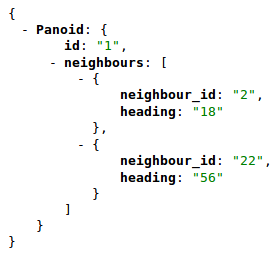
\includegraphics[width=0.4\textwidth]{ScreenshotAPIBeispiel.png}
\caption[API Beispiel]{Bildschirmfoto des gegebenen API Beispiels}
\label{fig:ScreenshotAPIBeispiel}
\end{figure}

Die Darstellung dieser Ausgabe wurde mit Hilfe eines Darstellungstools auf
bessere Lesbarkeit optimiert. Im Normalfall würde die Ausgabe in einer Zeile
dargestellt werden. Dies zeigt wiederum, dass das Ausgabeformat nicht auf
menschliche Lesbarkeit ausgelegt ist.

Nachdem das ausgebende System der Beispielschnittstelle implementiert wurde,
soll dieses nachfolgend angefragt und die Antwort des Systems ausgewertet
werden. Die Anfrage an das System erfolgt, wie bereits erwähnt, asynchron
innerhalb einer Javascript-Funktion. Asynchron bedeutet hierbei, dass die
Anfrage unabhängig von dem Aufbau der restlichen Seite ausgeführt wird.
Unabhängig von der aktuell dargestellten Seite wird eine Anfrage ausgeführt,
dessen Ergebnis in die bereits dargestellte Seite integriert wird.

In \verweis{Prototyp} wurde bereits die Funktion "`createCustomLink"' aus dem
\anhang{AnhangJavascriptPrototyp}
(\nameref{sec:AnhangJavascriptPrototyp}) vorgestellt. In dieser Funktion
werden die Links festgelegt, die letzenendes die Navigationspfeile in der
Benutzeransicht abbilden. Im \verweis{Prototyp} wurden diese Links statisch
gesetzt. Nachfolgend soll der Prototyp in der Weise abgeändert werden, dass die
Links durch Aufrufen der API dynamisch festgelegt werden. Dazu wird die Funktion
\textit{createCustomLink} zunächst um einen Funktionausruf der Funktion
"`getPanoJson"' erweitert. Diese Funktion ist dafür zuständig, die oben
definierte API mit einer übergebenen ID anzufragen und ein JSON-Objekt an die
aufrufende Methode zurückzuliefern. Die Implementierung dieser Funktion ist in
\listing{Dynamisch_Nachbarn_nachladen} dargestellt.

\clearpage

\lstinputlisting[language=JavaScript,caption={Dynamisch Nachbarn
nachladen},label={lst:Dynamisch_Nachbarn_nachladen}]{Listings/Dynamisch_Nachbarn_nachladen.js}

Die Funktion \textit{getPanoJson} wird in Zeile 5 aufgerufen und fragt daraufhin
über einen sogenannten \textit{XMLHttpRequest} die oben genannte URL an (Zeile
25). Da die Antwort als unformartiertes Textdokument erfolgt und es nicht
möglich ist per HTTP Objekte zu übertragen muss die Antwort zunächst in ein
JSON-Objekt umgewandelt werden. Man spricht dabei von "`parsen"' (Zeile 28). Die
Elemente des zurückgelieferten JSON-Objektes (Zeile 30) können daraufhin von der
aufrufenden Funktion referenziert werden. Über "`pano.neighbours"' (Zeile 7)
erhält man beispielsweise eine Liste aller Nachbarn, die im oben dargestellten
Quellcode durchlaufen und in die \textit{Links}-Liste geschrieben werden (Zeile
8ff.).

Durch die Erweiterung des Prototyps ist dieser in der Lage, die im
Administrationsbereich gepflegten Daten dynamisch abzurufen.

An dieser Stelle des Entwicklungsprozesses sind die Funktionen des
Administrationsbereichs vollständig umgesetzt und die Benutzeransicht greift
über APIs dynamisch auf die hinterlegten Informationen zu. Die Umsetzung des
Projektes ist damit abgeschlossen.